\section{Model-to-Tree Transformation with SDMs}


\begin{enumerate}
    
\item[$\blacktriangleright$] \texttt{transformLibraries()~:Folder}
  (Fig.~\ref{fig:moca-transformLibraries})    
  %\usepackage{graphics} is needed for \includegraphics
\begin{figure}[!htbp]
\begin{center}
 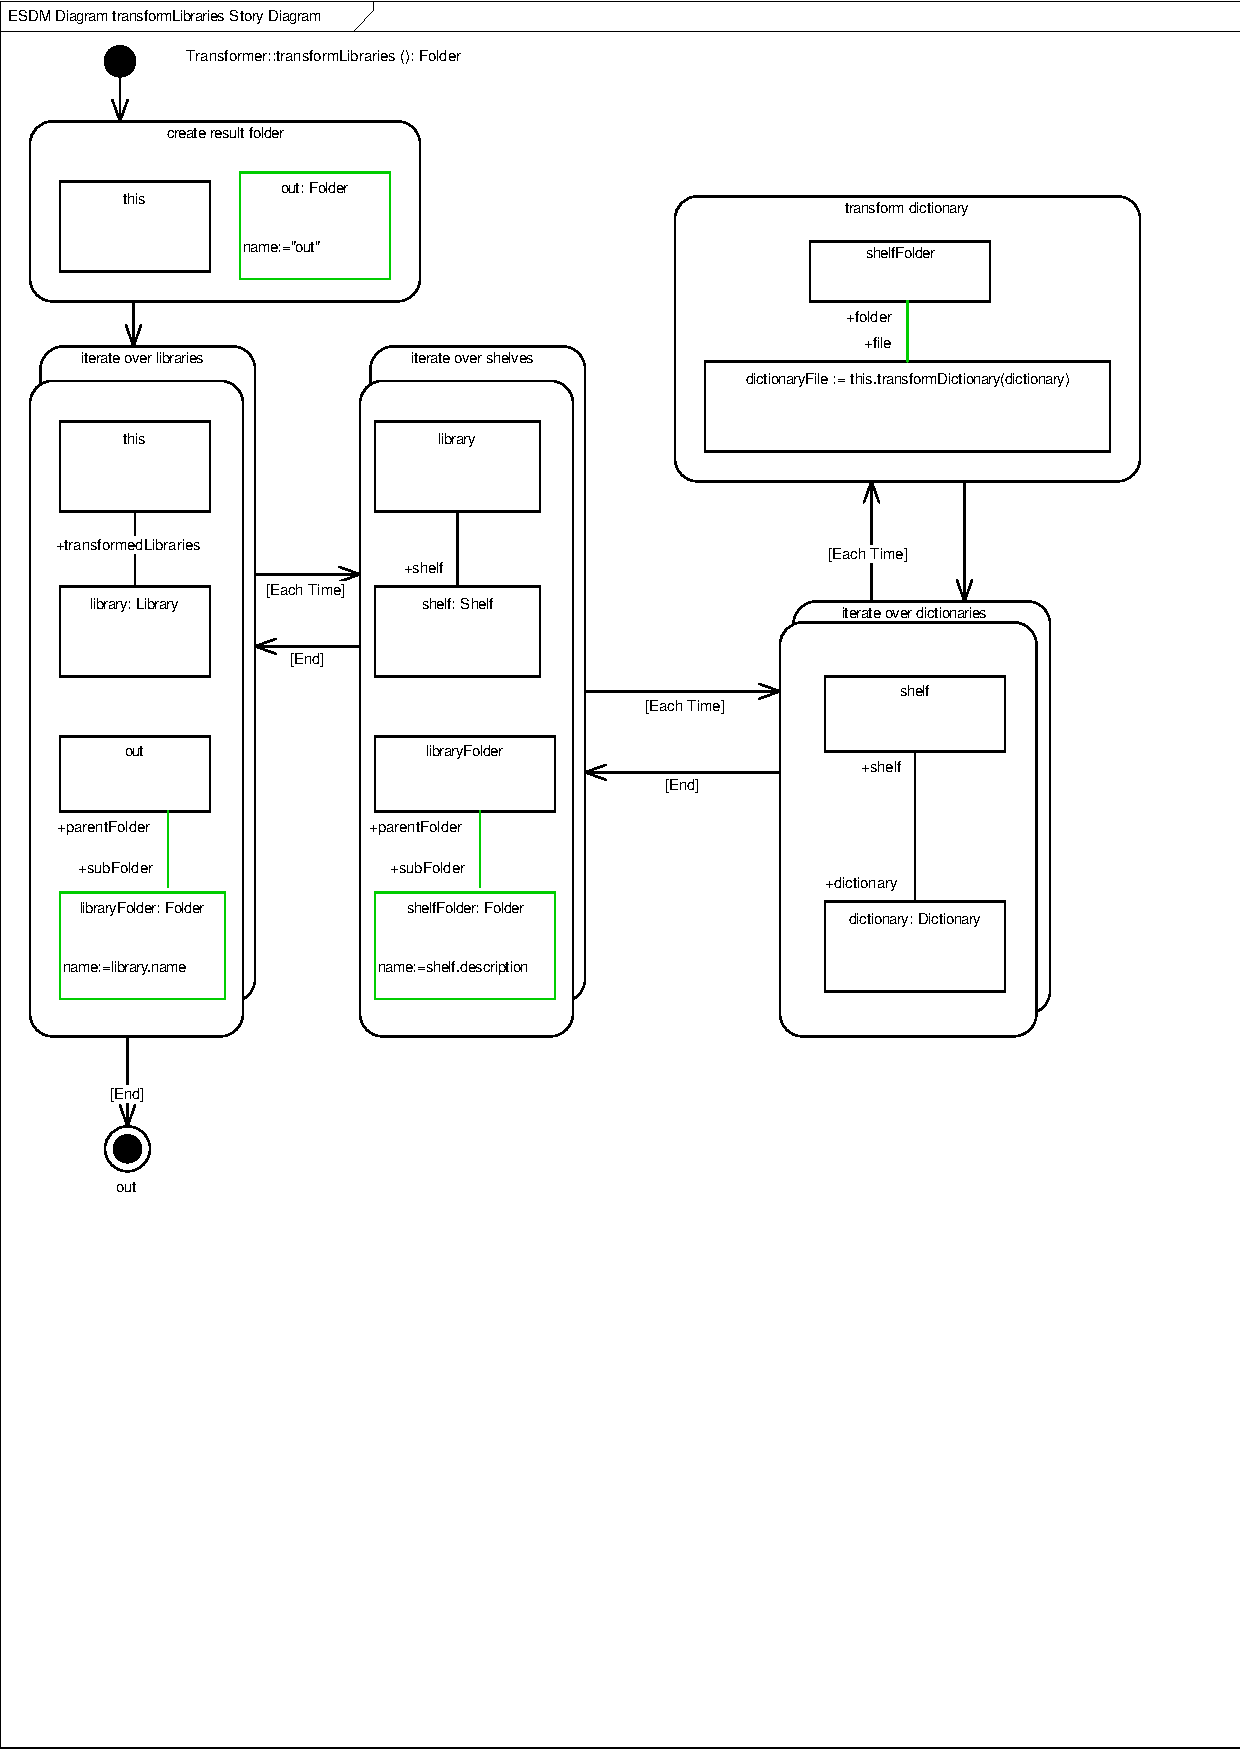
\includegraphics[width=\textwidth]{pics/moca/4ModelToMocaTree/transformLibraries}
  \caption{Iterate over all libraries} 
  \label{fig:moca-transformLibraries}
\end{center}
\end{figure}

\item[$\blacktriangleright$] \texttt{transformLibrary(Library)~:Folder}
  (Fig.~\ref{fig:moca-transformLibrary})    
  %\usepackage{graphics} is needed for \includegraphics
\begin{figure}[!htbp]
\begin{center}
 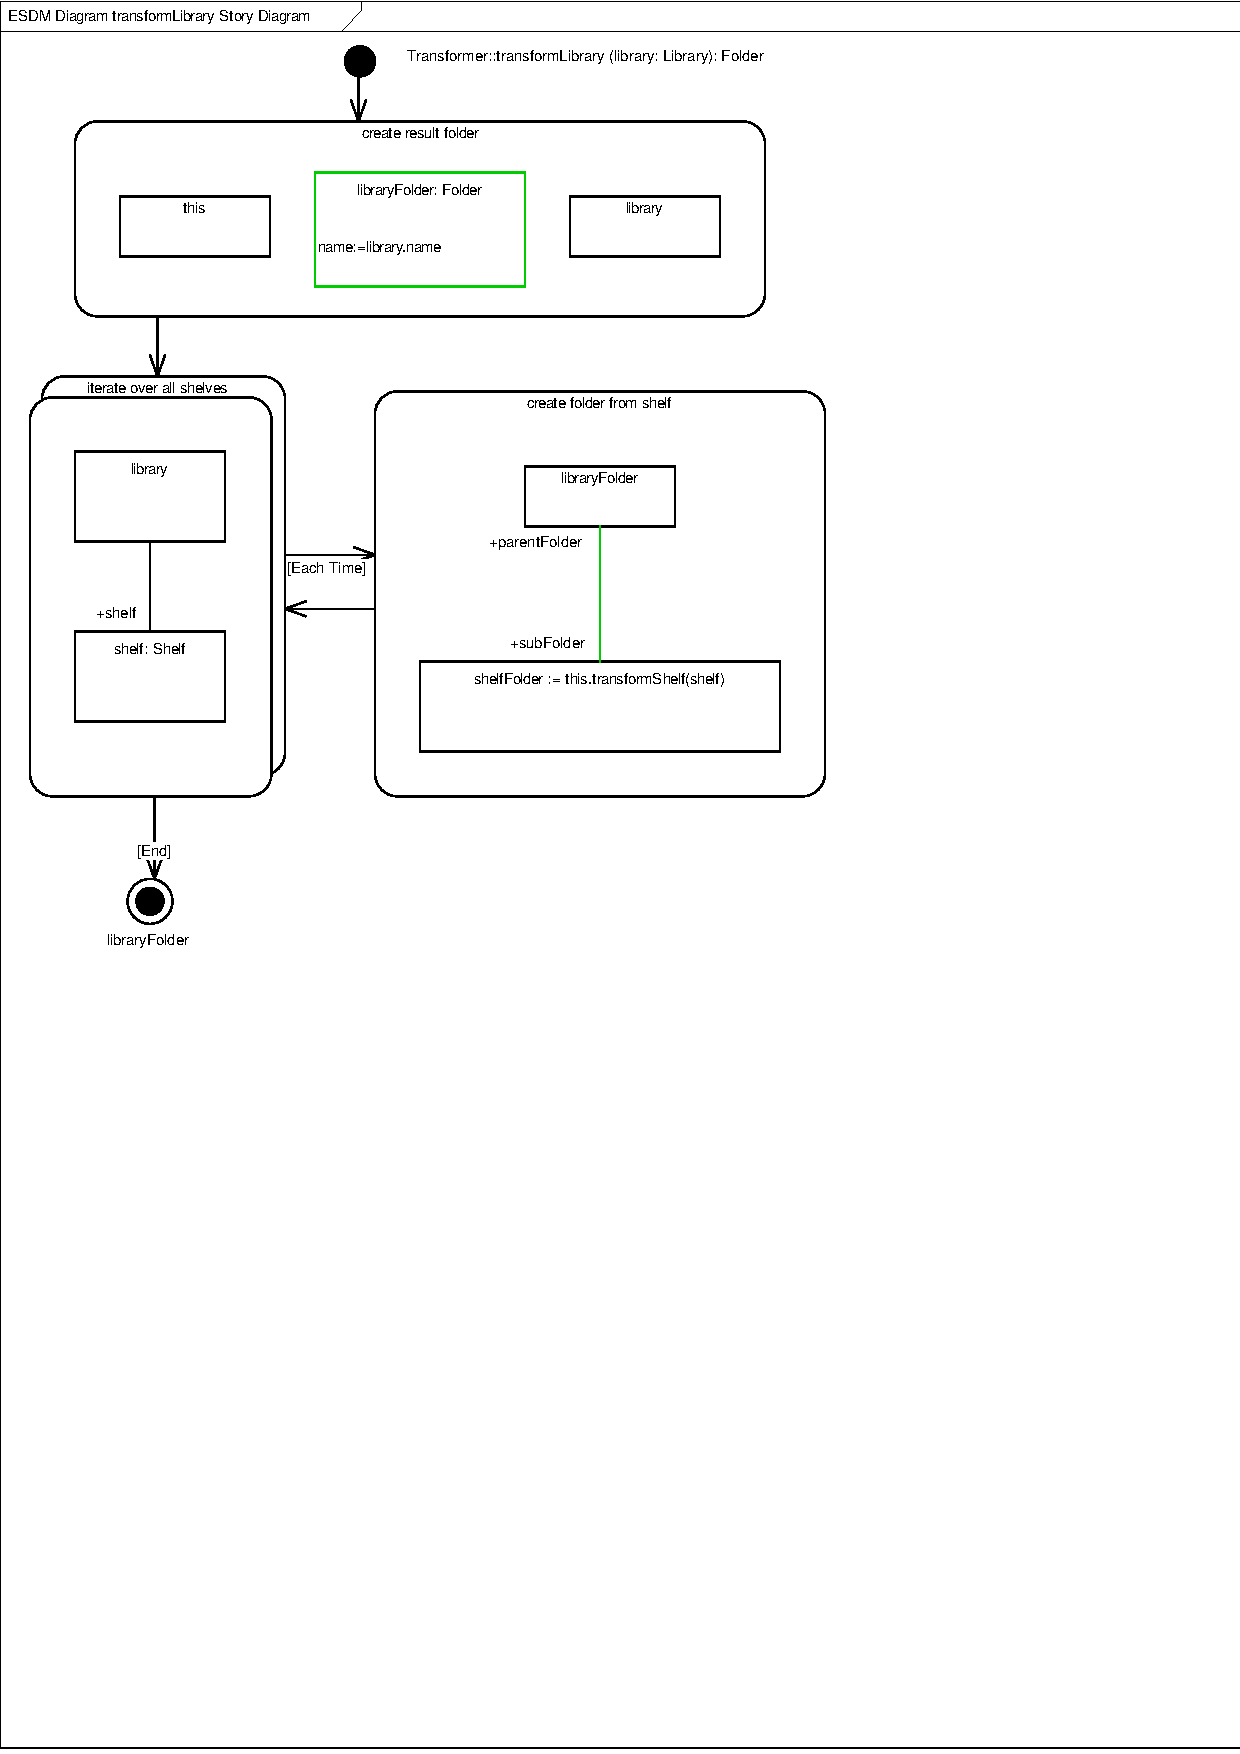
\includegraphics[width=\textwidth]{pics/moca/4ModelToMocaTree/transformLibrary}
  \caption{Transform the given library into a folder} 
  \label{fig:moca-transformLibrary}
\end{center}
\end{figure}
  
\item[$\blacktriangleright$] \texttt{transformShelf(Shelf)~:Folder}
  (Fig.~\ref{fig:moca-transformShelf})    
  %\usepackage{graphics} is needed for \includegraphics
\begin{figure}[!htbp]
\begin{center}
 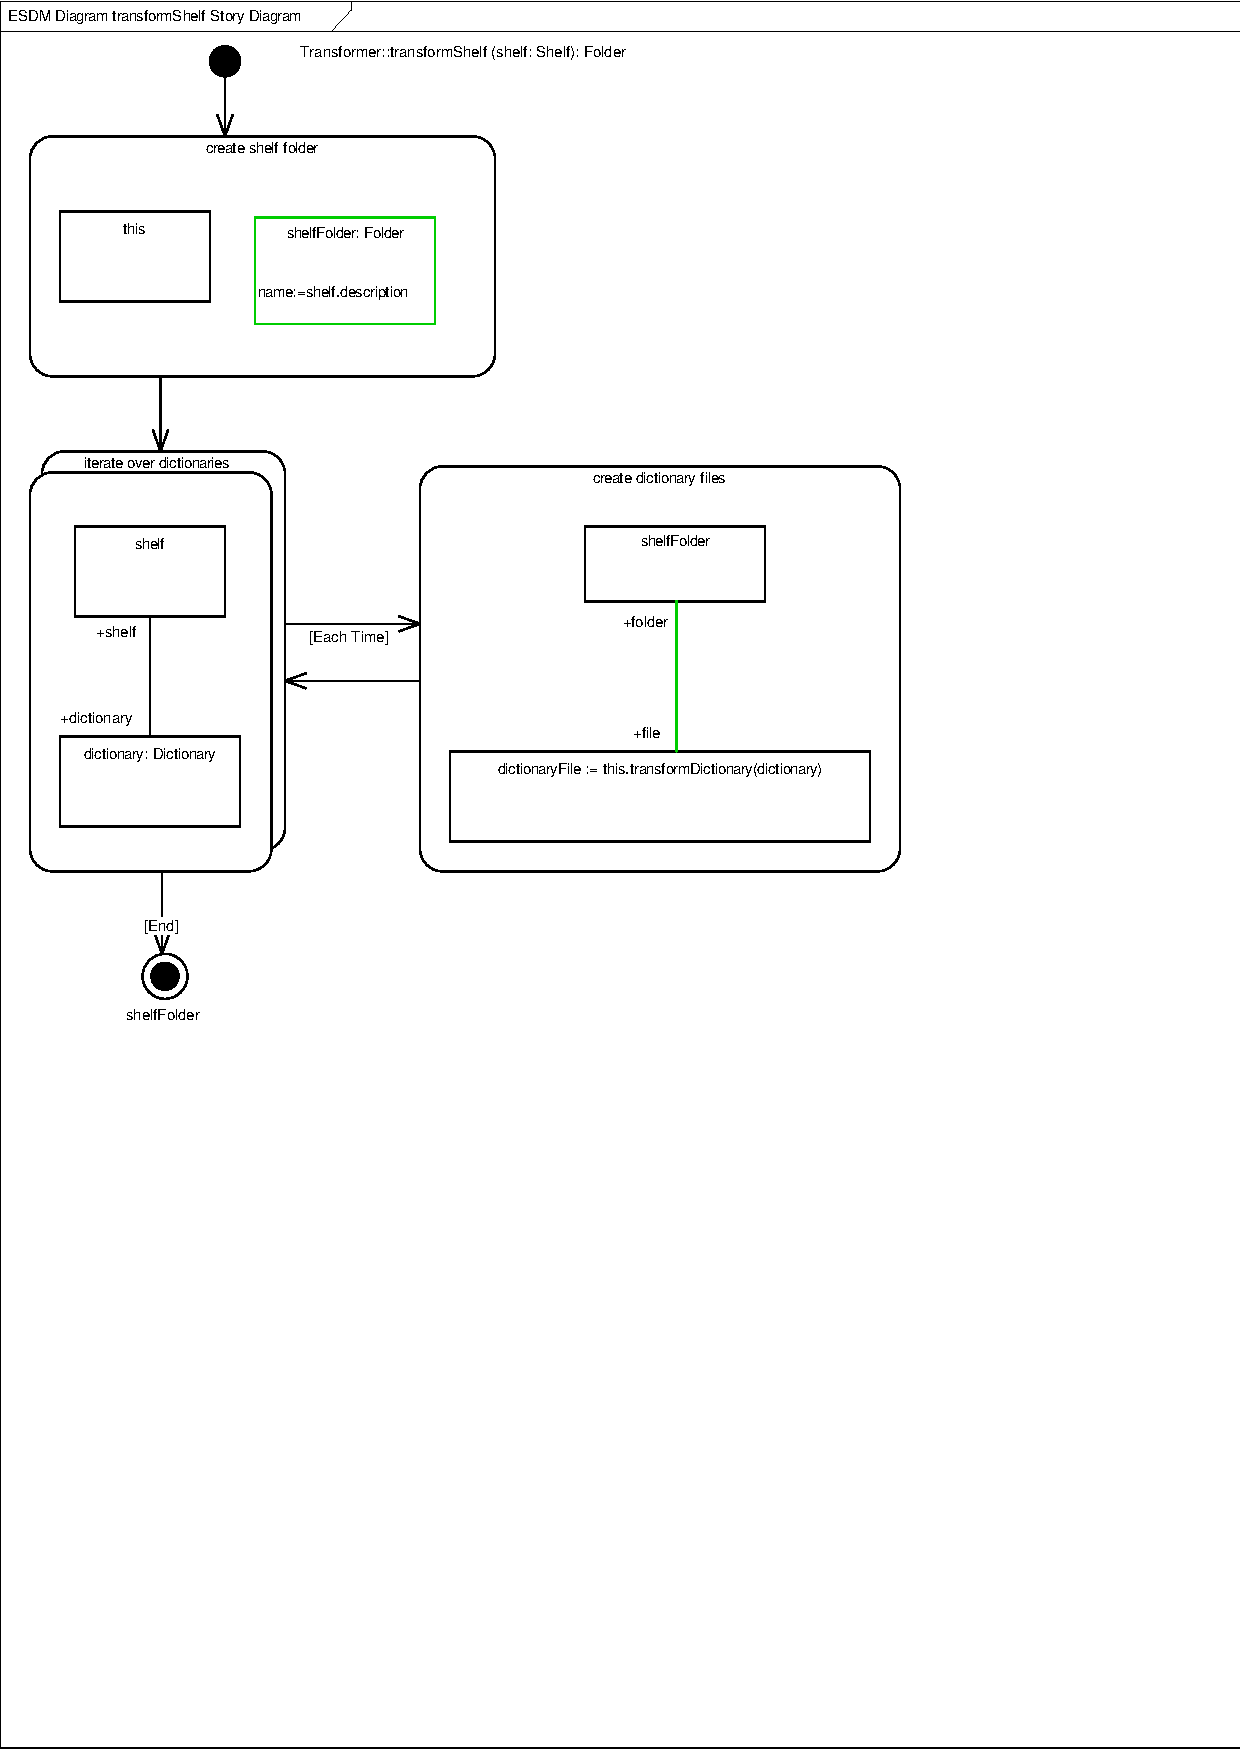
\includegraphics[width=\textwidth]{pics/moca/4ModelToMocaTree/transformShelf}
  \caption{Transform the given shelf into a folder} 
  \label{fig:moca-transformShelf}
\end{center}
\end{figure}

\item[$\blacktriangleright$] \texttt{transformDictionary(Dictionary)~:File}
  (Fig.~\ref{fig:moca-transformDictionary})    
  %\usepackage{graphics} is needed for \includegraphics
\begin{figure}[!htbp]
\begin{center}
 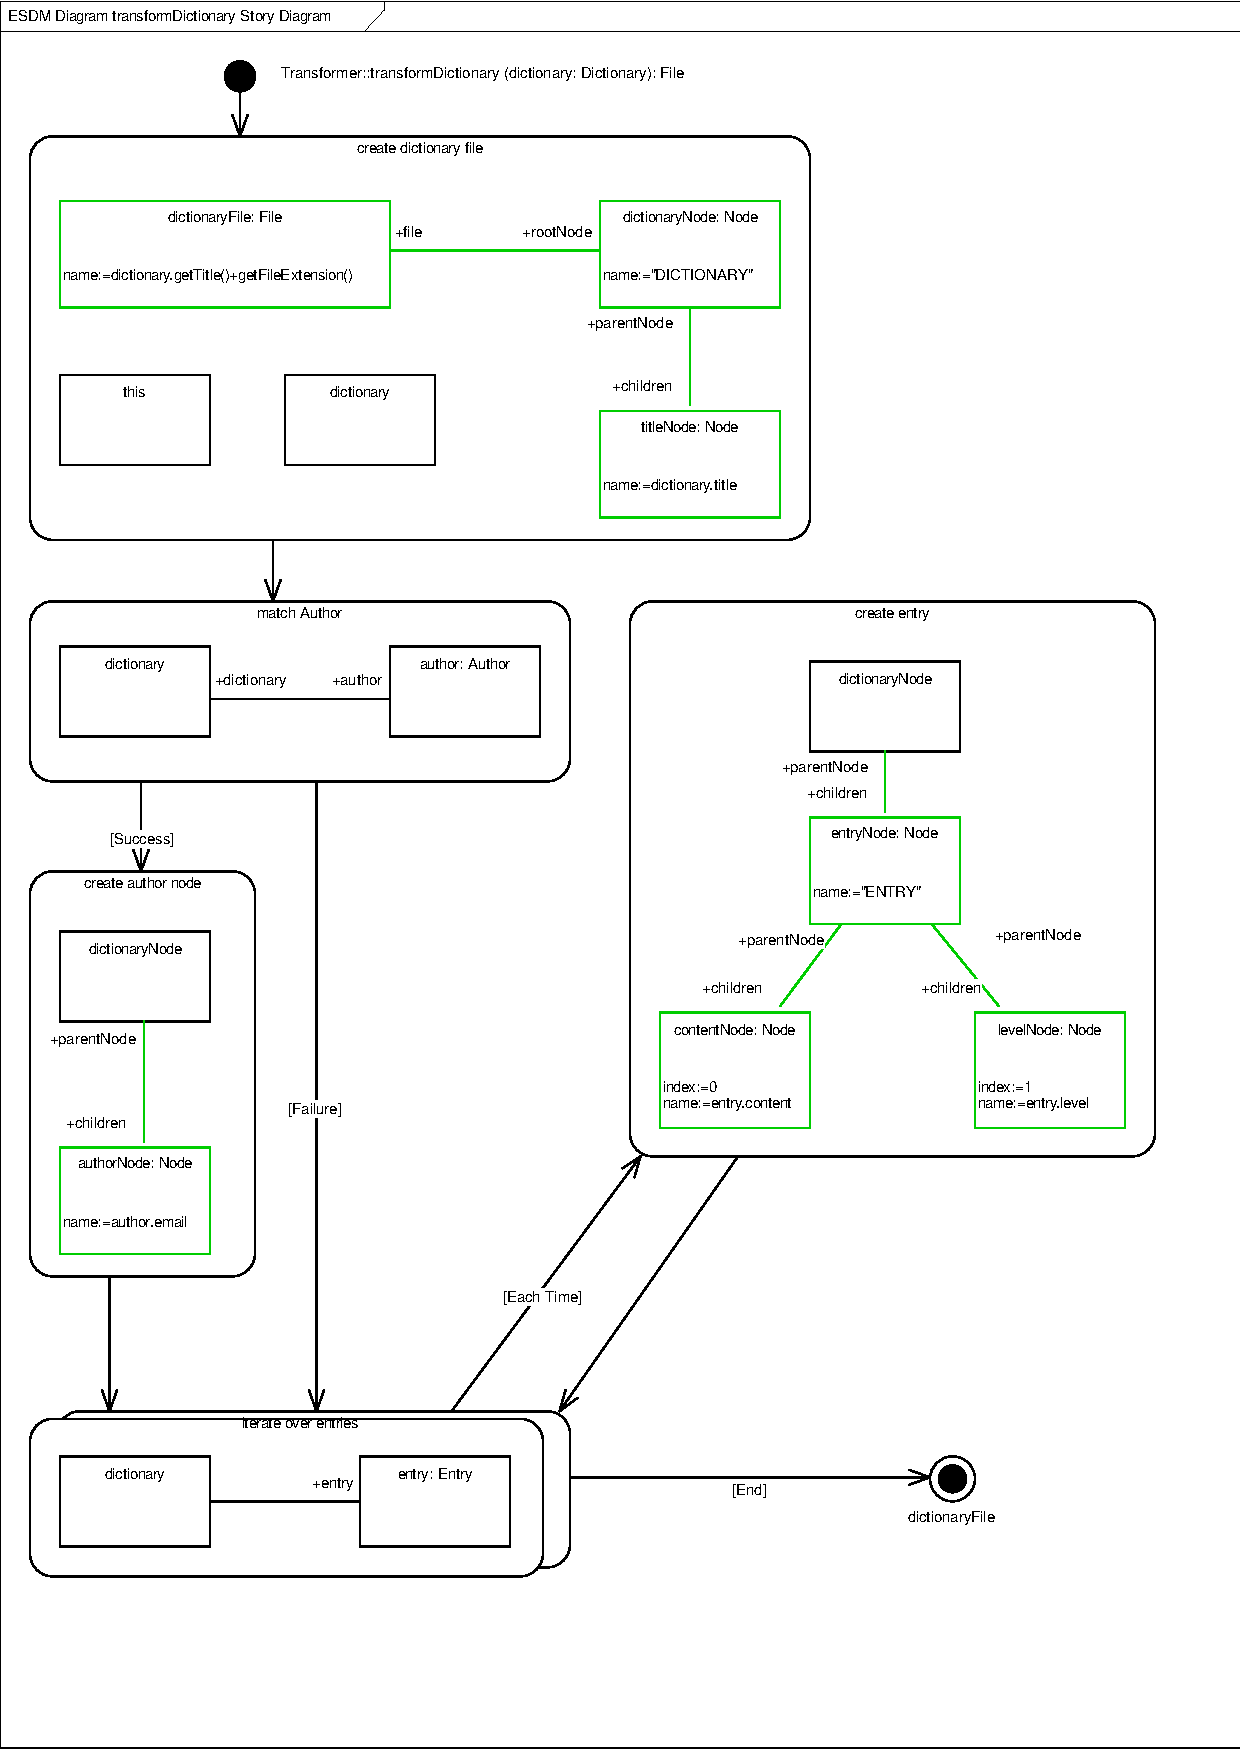
\includegraphics[width=\textwidth]{pics/moca/4ModelToMocaTree/transformDictionary}
  \caption{Create a file from the given dictionary} 
  \label{fig:moca-transformDictionary}
\end{center}
\end{figure} 


\item[$\blacktriangleright$] As a final step, open \texttt{MocaMain.java}
(Fig.~\ref{fig:moca-8-MocaMain}) and add the following lines:
\begin{verbatim}
// Perform model-to-tree 
Folder out = transformer.transformLibraries();
\end{verbatim}
\end{enumerate}